\documentclass{article}
\linespread{1.25}

\usepackage[top = 2cm, right=2cm, left=2cm]{geometry}
\usepackage{graphicx}
\usepackage[section]{placeins}
\usepackage[hidelinks, urlcolor=blue]{hyperref}
\usepackage{float} % for image position in exatly where you want
\usepackage[perpage, stable]{footmisc}
\usepackage{interval}

\usepackage{xepersian}
\settextfont{B Nazanin}
\setlatinmonofont{CMU Serif}
%\setlatinmonofont{Times New Roman}
\setlatintextfont{Times New Roman}

% Set Latin Modern font for the bullets in itemizea
\newfontfamily\latinbullet{Latin Modern Roman}



\title{گزارش تکلیف 
	\lr{ID3 Algorithm}
}
\author{درس یادگیری ماشین}
\date{
	امیرحسین ابوالحسنی\\
	400405003
}


% Commands
\newcommand{\column}[1]{\lr{\textit{#1}}}
\renewcommand{\labelitemi}{{\latinbullet\textbullet}} % Use the bullet from Latin Modern font

\begin{document}
	\maketitle
	\newpage
	\tableofcontents
	\newpage
	\section{مقدمه}
	درخت تصمیم گیری یک مدل یادگیری نظارت شده است که به طور گسترده ای در مسائل طبقه‌بندی مورد استفاده قرار می‌گیرد.
	الگوریتم \lr{ID3} یکی از پرکاربرد ترین الگوریتم‌های ساخت درخت تصمیم می باشد. این الگوریتم با استفاده از معیار انتروپی
	\footnote{\lr{Entropy}}
	بهترین ویژگی را برای تقسیم گره انتخاب می کند و به طور بازگشتی این فرایند را تا زمان رسیدن به یکی از شرط‌های پایه انجام می‌دهد.\\
	در این گزارش، ابتدا به بررسی دیتاست و پیش پردازش های روی آن پرداخته می‌شود، سپس توضیحی درباره شیوه 
	\lr{Feature Selection}
	داده می‌شود و در نهایت، نتایج هر درخت روی زیرمجموعه‌ای از ویژگی‌ها بررسی می گردد.
	
	\section{بررسی دیتاست}
	\subsection{آشنایی با ویژگی‌ها}
	در این تکلیف دیتاست با نام 
	\lr{Salary}
	مورد استفاده قرار می‌گیرد. این دیتاست متشکل از 32561 نمونه، 15 ویژگی افراد را همراه با کلاس درامد سالانه‌شان ثبت کرده است.
	
	\begin{table}[h]
		\centering
		\begin{tabular}{|c|c|c|c|}
			\hline
			نام ویژگی &‌ نوع ویژگی & تعداد مقادیر یکتا & نمونه مقدار\\
			\hline
			\hline
			\column{age} & عددی &  & 50\\
			\hline
			\column{workclass} & گسسته & 9 & \lr{Federal-gov}\\
			\hline
			\column{fnlwgt} & عددی &  & 77516\\
			\hline
			\column{education} & گسسته & 16 & \lr{HS-grad}\\
			\hline
			\column{education-num} & گسسته & 16 & 3\\
			\hline
			\column{marital-status} & گسسته & 7 & \lr{Married-spouse-absent}\\
			\hline
			\column{occupation} & گسسته & 15 & \lr{Tech-support}\\
			\hline
			\column{relationship} & گسسته & 6 & \lr{Wife}\\
			\hline
			\column{race} & گسسته & 5 & \lr{White}\\
			\hline
			\column{sex} & گسسته & 2 & \lr{Male}\\
			\hline
			\column{capital-gain} & عددی &  & 10566\\
			\hline
			\column{capital-loss} & عددی &  & 974\\
			\hline
			\column{hours-per-week} & عددی &  & 88\\
			\hline
			\column{native-country} & 4گسسته & 2 & \lr{England}\\
			\hline
			\column{salary} & 2گسسته & 2 & \lr{<=50K, >50K}\\
			\hline
		\end{tabular}
		\caption{ویژگی‌های دیتاست \lr{salary}}
	\end{table}
	\subsection{مقادیر هیچ مقدار}
	خوشبختانه این دیتاست داری هیج سلول گم شده‌ای نمی‌باشد.
	\newpage
	\subsection{نمودار‌ها}
	توزیع برخی ویژگی‌ها در دیتاست برسی شده است.\\
	همانطور که در نمودار 
	\ref{fig: sex dist}
	می‌توان دید، که جمعیت مردان دو برابر جمعیت زنان در این دیتاست می باشد.
	\begin{figure}[H]
		\centering
		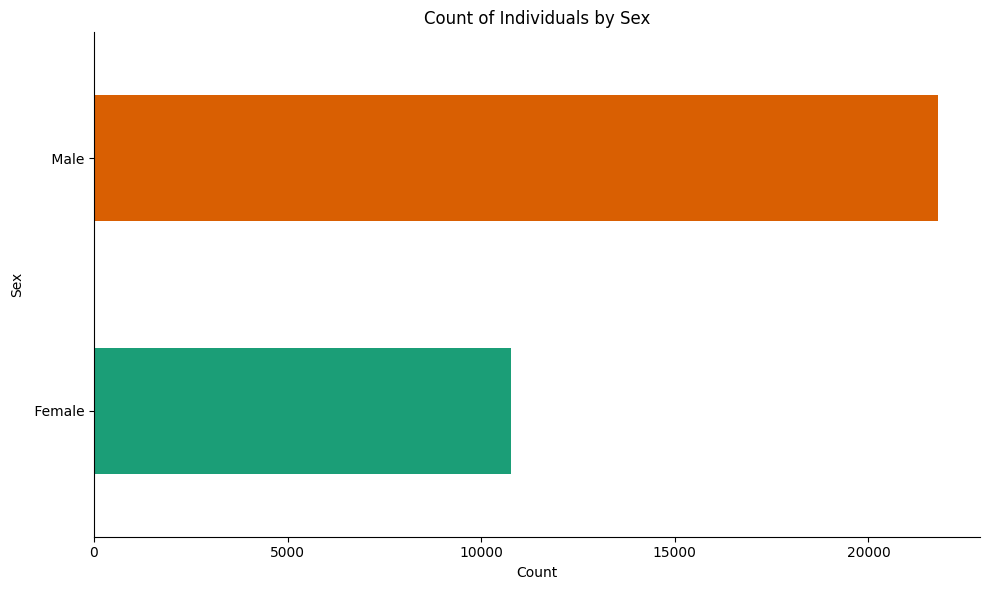
\includegraphics[scale=0.5]{figs/sex_dist}
		\caption{
			توزیع ویژگی 
			\lr{Sex}
		}
		\label{fig: sex dist}
	\end{figure}
			یکی از ویژگی‌های دیگر، نژاد هر نمونه در دیتاست می‌باشد، همانطور که در نمودار
			\ref{fig: race dist}
			 مشاهده می شود، افراد سفید پوست بیشترین افراد و افراد هندی-اسکیمو کمترین نژاد مشخص در این دیتاست هستند.
	\begin{figure}[H]
		\centering
		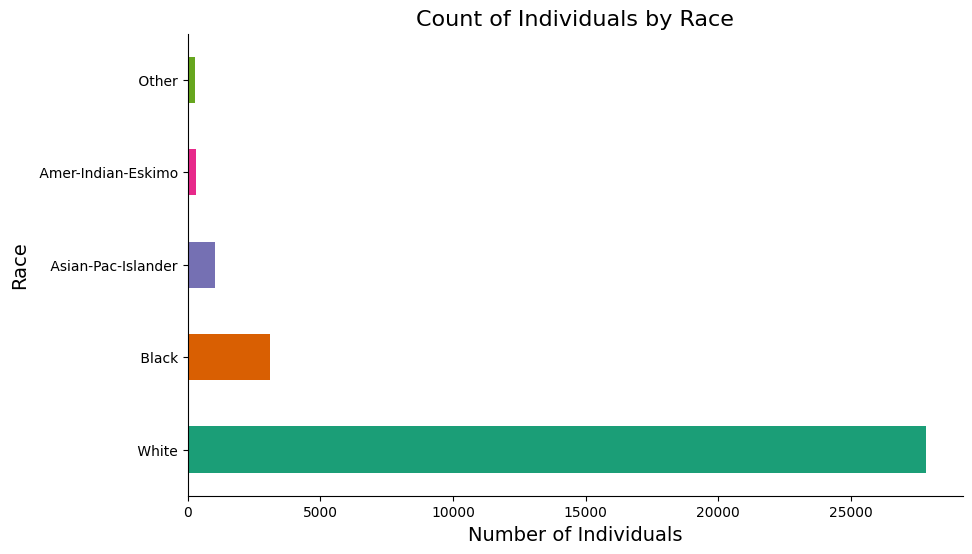
\includegraphics[scale=0.5]{figs/Race_dist}
		\caption{
			توزیع ویژگی 
			\lr{Race}
		}
		\label{fig: race dist}
	\end{figure}
	یکی از مهمترین توزیع‌های این دیتاست، توزیع متغیر 
	\lr{Age}
	می‌باشد. همانظور که در نمودار 
	\ref{fig: age dist}
	مشاهده می‌شود، بیشتر نمونه‌ها در 30 تا 40 سالگی خود قرار دارند. و همچنین افراد زیر 10 سال و بالای 90 سال عضویت بسیار کمی در این دیتاست دارند.\\
	\begin{figure}[H]
		\centering
		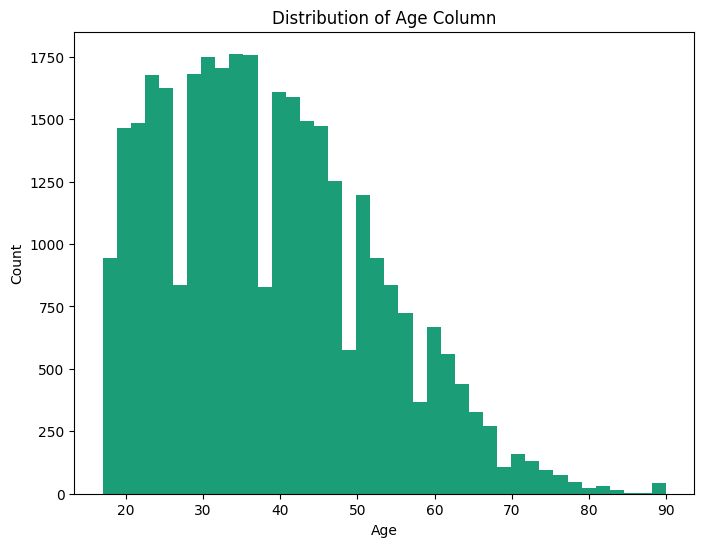
\includegraphics[scale=0.5]{figs/age_dist}
		\caption{
			توزیع ویژگی 
			\lr{Age}
		}
		\label{fig: age dist}
	\end{figure}
	همچنین توزیع ویژگی‌های افزایش سرمایه و کاهش سرمایه را در نمودارهای 
	\ref{fig: captial gain}
	و
	\ref{fig: captial loss}
	 می‌توان بررسی کرد. با توجه به ارتباط مالی با موضوع به نظر می‌رسد ویژگی‌های مرتبطی به تارگت باشند.
	\begin{figure}[H]
		\centering
		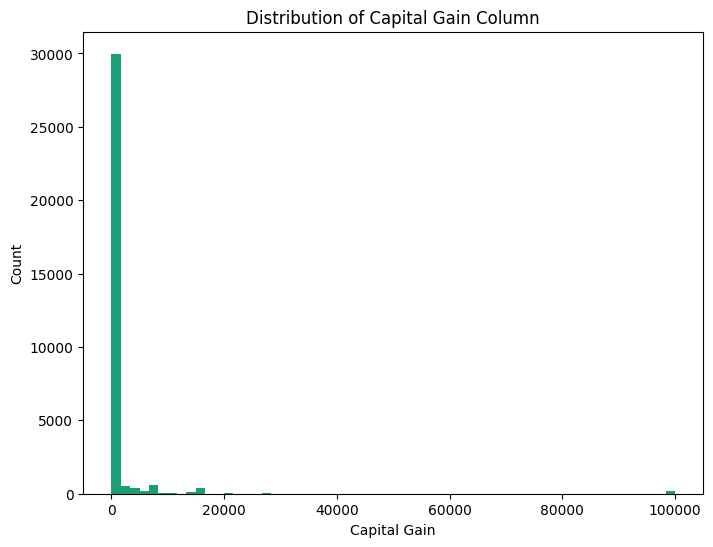
\includegraphics[scale=0.5]{figs/capital_gain_dist}
		\caption{
			توزیع ویژگی 
			\lr{Capital Gain}
		}
		\label{fig: captial gain}
	\end{figure}
	\begin{figure}[H]
		\centering
		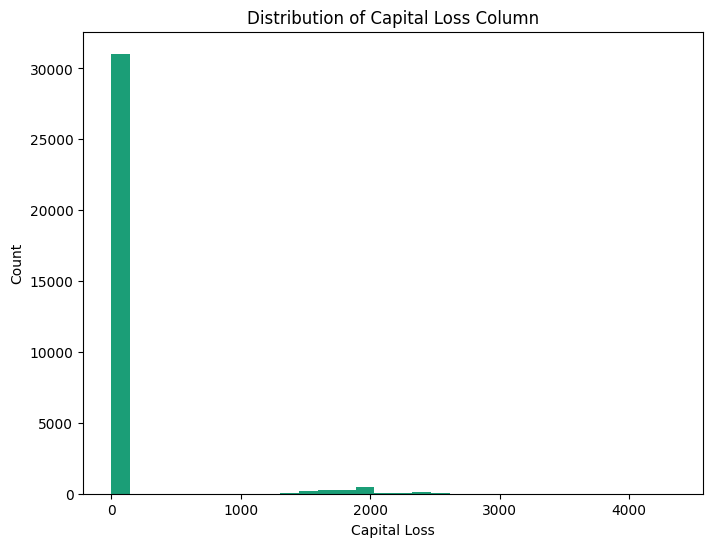
\includegraphics[scale=0.5]{figs/capital_loss_dist}
		\caption{
			توزیع ویژگی 
			\lr{Capital Loss}
		}
		\label{fig: captial loss}
	\end{figure}
	یکی دیگر از ویژگی‌های مهم سطح تحصیلات فرد است که در کشور‌هایی که روابط منطق تا حد قابل قبولی در آن برقرار است! ، معمولا افرادی که سطح بالاتری از تحصیلات را دارا هستند جزو افرادی هستند که درامد خوبی دارند (نمودار 
	\ref{fig: salary by education dist}
	)،‌ هرچند عکس این مورد صحیح نمی‌باشد.\\
	\begin{figure}[H]
		\centering
		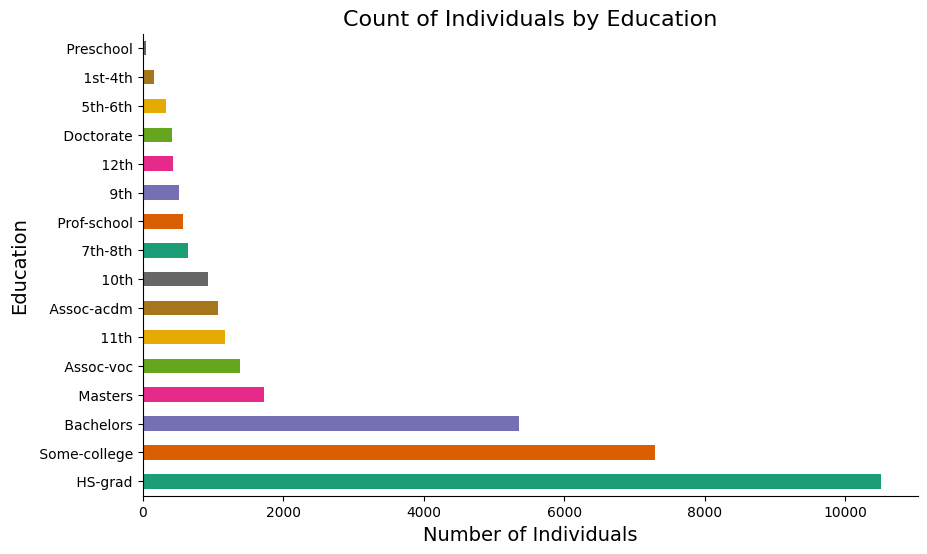
\includegraphics[scale=0.5]{figs/education_dist}
		\caption{
			توزیع ویژگی 
			\lr{Education}
		}
		\label{fig: education dist}
	\end{figure}
	\begin{figure}[H]
		\centering
		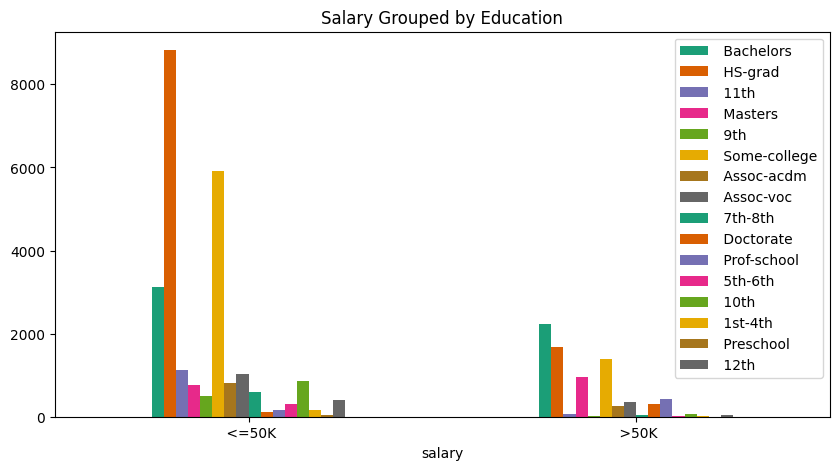
\includegraphics[scale=0.5]{figs/salary_by_edu}
		\caption{
			توزیع ویژگی 
			\lr{Salary}
			بر اساس
			\lr{Education}
		}
		\label{fig: salary by education dist}
	\end{figure}
	همچنین توزیع ساعت کار روزانه نمونه‌ها در نمودار 
	\ref{fig: hours dist}
	نشان داده شده است.\\
	\begin{figure}[H]
		\centering
		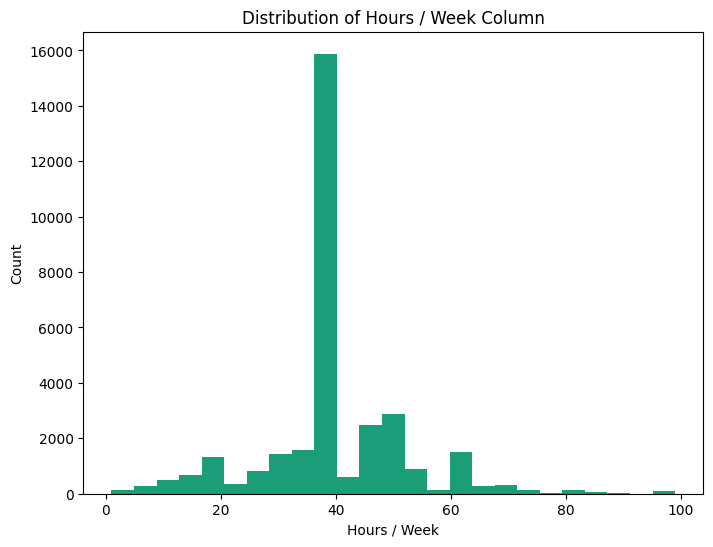
\includegraphics[scale=0.5]{figs/hours_dist}
		\caption{
			توزیع ویژگی 
			\lr{Hours Per Week}
		}
		\label{fig: hours dist}
	\end{figure}
	از دیگر ویژگی‌های تقریبا مرتبط می‌توان به نوع شغل افراد اشاره کرد که توزیع آن در نمودار 
	\ref{fig: occ dist}
	نشان داده شده است.\\
	\begin{figure}[H]
		\centering
		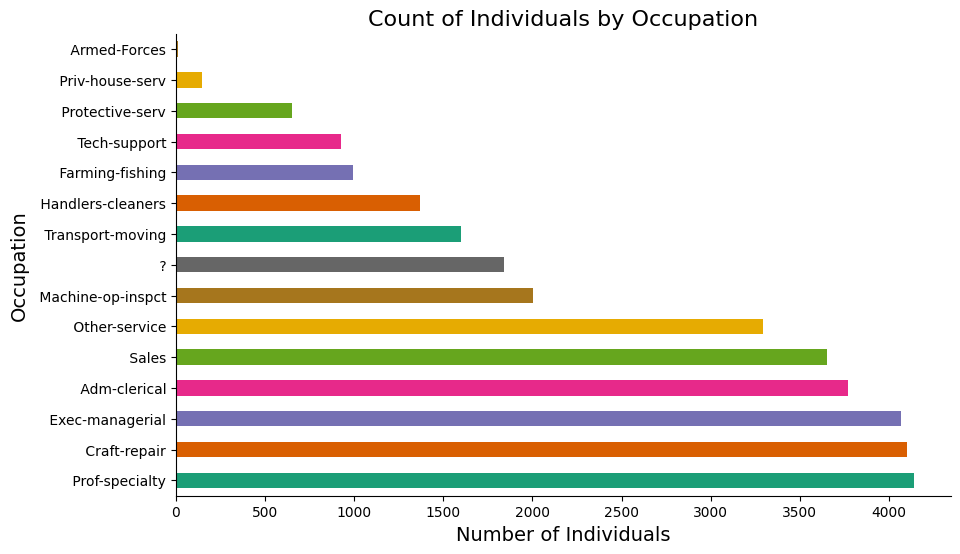
\includegraphics[scale=0.5]{figs/occupation_dist}
		\caption{
			توزیع ویژگی 
			\lr{Occupation}
		}
		\label{fig: occ dist}
	\end{figure}
	یکی از ویژگی‌های کلیدی که بعدا توسط درخت به دست می‌آید، ویژگی 
	\lr{Relationship}
	می باشد.(نمودار 
	\ref{fig: relationship dist}
	)
	\begin{figure}[H]
		\centering
		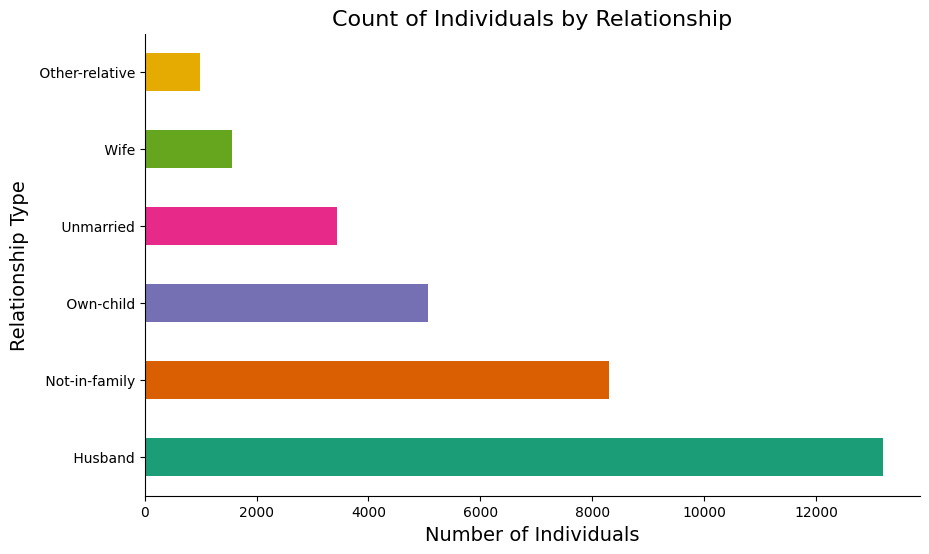
\includegraphics[scale=0.5]{figs/relationship_dist}
		\caption{
			توزیع ویژگی 
			\lr{Relationship}
		}
		\label{fig: relationship dist}
	\end{figure}
	در انتها برای جمع بندی نمودارها سعی شده توزیع کلاس‌های ویژگی هدف بررسی شود. همانطور که مشاهده می‌شود، دیتا ست به هیچ وجه بالانس نمی‌باشد و داده‌های کلاس ‌مینور
	\footnote{\lr{Minor}}
	مربوط به کلاس درامد بالاتر می‌باشد.\\
	همچمنین در نمودار
	\ref{fig: salary grouped}
	توزیع کلاس هدف با توجه به سه ویژگی نشان داده شده تا درک بهتری از رابطه هر ویژگی با هر کلاس ویژگی هدف به دست بیاید.
	
	\begin{figure}[H]
		\centering
		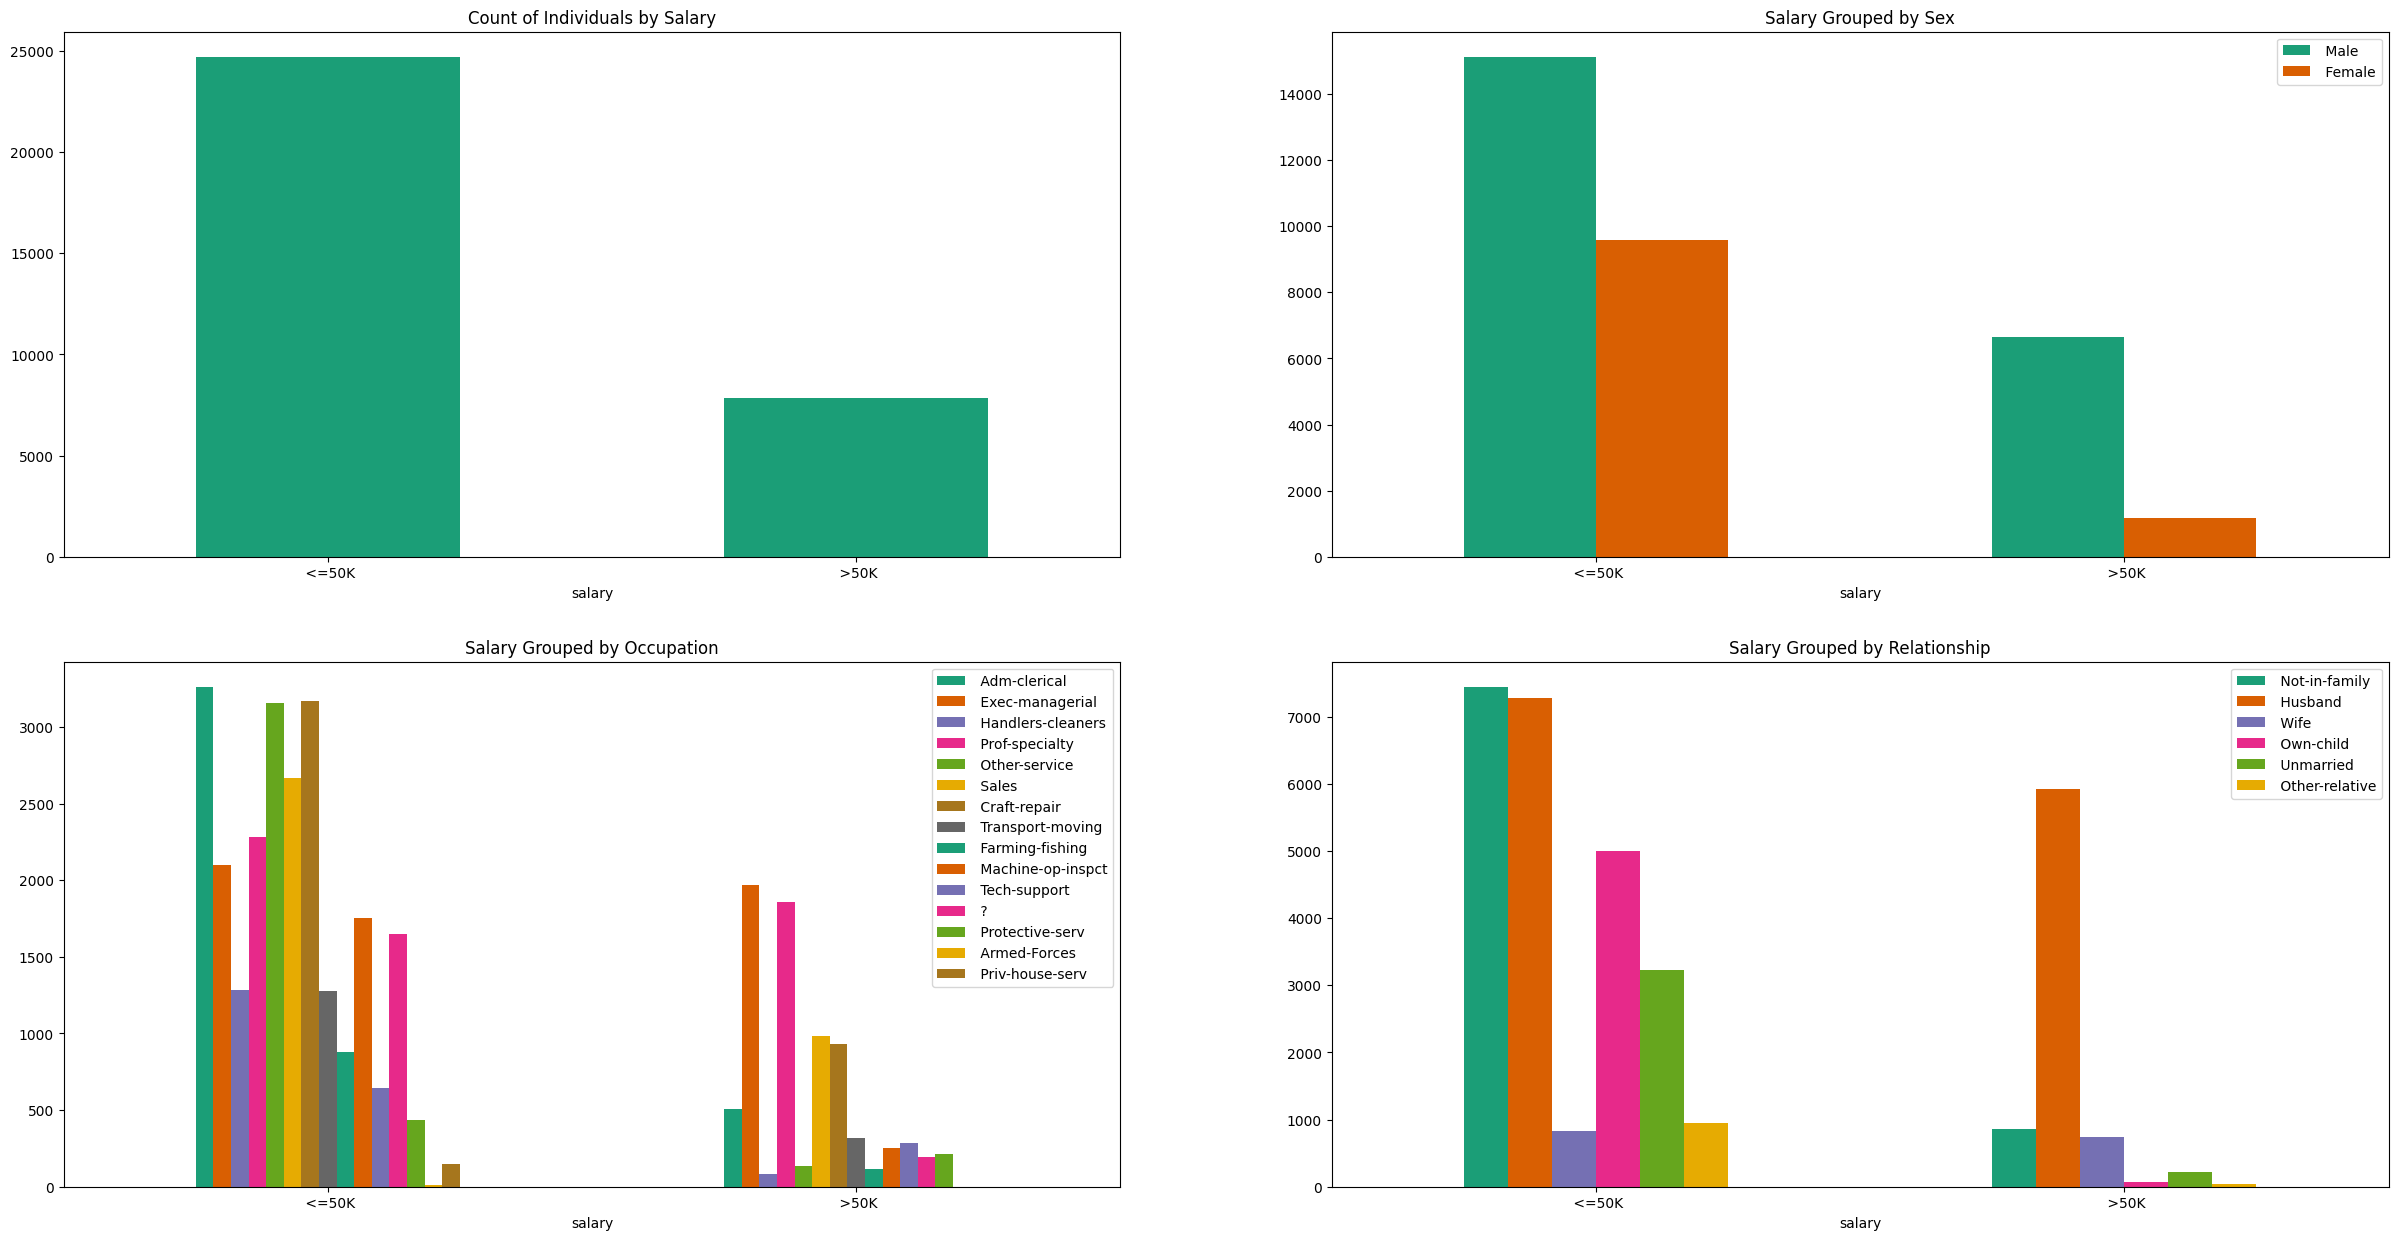
\includegraphics[scale=0.3]{figs/Salary_grouped_dist}
		\caption{
			توزیع ویژگی 
			\lr{Salary}
			طبق ویژگی‌های 
			\lr{Occupation, Relationship, Sex}
		}
		\label{fig: salary grouped}
	\end{figure}
	\FloatBarrier
	\subsection{دسته بندی ویژگی‌ها}
	برای کار با درخت تصمیم نیاز به این است که داده‌ها گسسته باشند. با تعیین بازه‌هایی، ویژگی‌های 
	\lr{Age, Hours per Week, Capital Gain}
	گسسته سازی شدند.\\
	در جدول 
	مقادیر هر ویژگی و بازه‌های گسسته‌سازی نشان داده شده است.
	\begin{table}
		\centering
		\begin{minipage}[t]{0.3\textwidth}
			\centering
			\begin{tabular}{|c|c|c|}
				\hline
				\[
				\interval{0}{30}
				\] &\[
				\interval[right]{31}{50}
				\]& \[
				\interval[right]{51}{\infty}
				\]\\
				\hline
				1 - 30 & 31 - 50 & \lr{Over 50}
			\end{tabular}
		\end{minipage}
	\end{table}
	
	
	\section{
		انتخاب ویژگی
		\footnote{\lr{Feature Selection}}
		‌}
	
	\section{آموزش مدل}
	
	\section{نتایج}
	
	\section{نتیجه گیری}
	
	\section{مراجع}
	
	
	
\end{document}